%\setcounter{section}{5}
\section{НЕЛИНЕЙНОЕ ПРОГРАММИРОВАНИЕ}
\subsection{Постановка задачи и общие понятия}
\indent\indent\textbf{\textit{1.Пример~ возникновения~ задачи~ нелинейного программирования~ в~ экономике}}. Пусть предприятие изготавливает два вида продукции \(P_1\) и \(P_2\). Если обозначить прибыль от реализации единицы продукции \(P_1\) через \(c_1\), а \(P_2\) — через \(c_2\), то суммарную прибыль предприятия можно записать в виде
   \[z = c_1x_1+c_2x_2, \]
где \(x_1\) и \(x_2\) - плановые количества продукции \(P_1\) и \(P_2\).

Предприятие стремится к максимуму функции \(z\) при ограничениях, определяемых условиями производства. Ранее  мы считали величины \(c_1\) и \(c_2\) константами, независящими от \(x_1\)  и \(x_2\). Однако такое предположение оправдано лишь при изменении\(x_1\)  и\(x_2\) в  некоторых пределах, да и то приближенно. Величины \(c_1\) и \(c_2\) зависят от \(x_1\)  и \(x_2\). Чем больше продукции попадает на рынок, тем меньше цены на эту продукцию. Предположим, что истинная прибыль от реализации единицы продукции \(P_1\) равна  $c_1-\cfrac{x_1}{b_1}$, а продукции P2 — $c_2-\cfrac{x_2}{b_2}$, где \(c_1\), \(b_1\) и \(c_2\), \(b_2\) —некоторые константы. Общая прибыль определяется формулой $$z=\left(c_1-\cfrac{x_1}{b_1}\right)x_1+\left( c_2-\cfrac{x_2}{b_2}\right)x_2$$

Эта целевая функция уже не является линейной, т.к. в ее выражении присутствуют квадраты переменных. Задача на максимум для такой функции уже не может быть решена методами линейного программирования.

\textbf{\textit{2.Общая ~ формулировка ~ задачи нелинейного программирования и связанные с ней общие понятия.}} Задачей нелинейного программирования мы будем называть задачу
\[z=f(x_1,x_2,\dots,x_n)\to\mathrm{max(min)};\]
\[
    \begin{cases}
        \varphi_1(x_1,x_2,\dots,x_n)=0 ,\\
        \varphi_2(x_1,x_2,\dots,x_n)=0,\\
        \dots\dots\dots\dots\dots\dots\dots\\\
        \varphi_k(x_1,x_2,\dots,x_n)=0,\\
        \varphi_{k+1}(x_1,x_2,\dots,x_n)\leq 0,\\
        \dots\dots\dots\dots\dots\dots\dots\\\
         \varphi_m(x_1,x_2,\dots,x_n)\leq0,\\
    \end{cases}
\]

В этой задаче часть ограничений является равенствами, а часть$-$\\неравенствами. Все входящие в формулировку функции могут быть нелинейными. В дальнейшем часто совокупность значений переменных \\$x_1,x_2,\ldots,x_n$ мы будем рассматривать как точку $\vec x.$ в \textit {n}-мерном евклидовом пространстве $ R{}^n\Biggl(\vec x\in R{}^n\Biggr).$ Множество точек \(R^n\) которые удовлетворяют системе ограничений задачи, обозначим через М. Сокращенно задачу можно записать так:
\[f(\vec x)\to\mathrm{max(min)}\]
\[\vec x\in \mathrm{M} \subset R{}^n\]
\indentОтметим, что конкретный вид системы ограничений можно изменять, не изменяя множества М, т.е. формулировать задачу в различных формах. Каждое равенство можно заменить системой неравенств
\[
    \begin{cases}
        \varphi_i(\vec x)\leqslant 0,\\
       -\varphi_i(\vec x)\leqslant 0.
    \end{cases}
\]

Поэтому можно считать, что система ограничений состоит только из неравенств. С другой стороны, каждое неравенство $\varphi_i(\vec x)\le 0$ можно заменить эквивалентным равенством~ $\varphi_i(\vec x)+x_{n+1}^2 =  0$~ вводя новую переменную $x_{n+1}$. Отметим, что в ~ нелинейном~ программировании словие неотрицательности переменной не играет особой роли и включается (если оно есть) в систему ограничений "на общих основаниях". Количество ограничений тоже можно изменить, не меняя, по сути, задачу. Например, всегда можно систему ограничений записать в виде одного равенства. Для этого вначале преобразуем систему ограничений в систему равенств
\[
    \begin{cases}
        \varphi_1(x_1,x_2,\dots,x_n)=0,\\
        \varphi_2(x_1,x_2,\dots,x_n)=0,\\
        \dots\dots\dots\dots\dots\dots\dots\\
        \varphi_m(x_1,x_2\dots,x_n)=0.\\
    \end{cases}
\]
Эта же система эквивалентна одному  уравнению
\[\Phi(x_1,x_2,\dots,x_n)=\sum\limits_{i=1}^m \varphi_i{}^2(x_1,x_2,\dots,x_n)=0\]

Здесь, однако, следует заметить, что такое уменьшение количества ограничений часто не упрощает, а усложняет решение задачи.

\opredelenie{Локальным минимумом задачи называется такая точка $\vec x{}^{(0)}$ удовлетворяющая системе ограничений $(\vec x^{(0)} \in M)$, для которой выполнено неравенство $f(\vec x{}^{0})\leqslant f(\vec x)$. Здесь $\vec x$ $-$ произвольная точка множества $M\cap K_{\varepsilon}(\vec x^{(0)})$, $K_{\varepsilon}(\vec x^{(0)})$ $-$ $\varepsilon$ - окрестность точки $\vec x^{(0)}$.}

Под $\varepsilon$ - окрестностью точки $\vec x{}^{(0)}$=$\Bigl\{x_{1}^0,x_{2}^0,\dots,x_{n}^0\Bigr\} $ понимается множество точек $\vec x$=$\Bigl\{x_1,x_2\dots,x_n\Bigr\}$ для которых
\[\sqrt{\Biggl(x_1-x_1^{0}\Biggr){}^2+\Biggl(x_2-x_2^{0}\Biggr){}^2+\dots+\Biggl(x_n-x_n^{0}\Biggr){}^2}<\varepsilon.\]
\indent\indent Другими словами, в точке локального минимума значение целевой функции не больше, чем во всех точках множества $M$ достаточно близких к точке $\vec x^{(0)}$.

Аналогично определяется понятие локального максимума, т.е. точки $\vec x^{(0)}$, для которой выполняется неравенство
\[f(\vec x{}^{0})\geqslant f(\vec x) \text{ при } \vec x \in M\cap K_{\varepsilon}(\vec x^{(0)}).\]



\opredelenie{~Глобальным~минимумом (максимумом) задачи называется точка $\vec x \in M$ для которой $f(\vec x^{(0)})\leqslant f(\vec x)(f(\vec x^{(0)})\geqslant f(\vec x))$ для любой точки $\vec x \in M$.}


Решением~ задачи нелинейного программирования является точка~ глобального~  минимума или максимума (экстремума). В настоящее время регулярных общих методов нахождения глобальных экстремумов не существует. Правда,~ существуют методы~  случайного~  и эволюционного поиска (генетические алгоритмы), которые дают, вообще говоря, приемлемое, а не оптимальное решение. Здесь мы рассматриваем методы нахождения точек локального экстремума. Эти методы особенно важны для так называемых \textit{одноэкстремальных задач}.


\opredelenie{Задача ~ на ~минимум ~ нелинейного программирования называется одноэкстремальной, если каждый  ее ~ локальный минимум одновременно является и глобальным. Аналогично понимается одноэкстремальность задачи на максимум.}


Всякая задача линейного программирования является одноэкстремальной.

\subsection{Метод множителей Лагранжая}
\indent\indent\textbf{1. Задача на условный экстремум. Необходимые условия экстремума}. Рассмотрим задачу нелинейного программирования с ограничениями равенствами:
\[z=f(x_1,x_2,\dots,x_n)\to\mathrm{max(min)};\]
\[
    \begin{cases}
        \varphi_1(x_1,x_2,\dots,x_n)=0,\\
        \varphi_2(x_1,x_2,\dots,x_n)=0,\\
        \dots\dots\dots\dots\dots\dots\dots\\
        \varphi_m(x_1,x_2\dots,x_n)=0.\\
    \end{cases}
\]
\indentБудем рассматривать в каждой точке $\vec x \in M$  $m+1$ вектор градиентов функций $f(x),\varphi_1(\vec x),\varphi_2(\vec x),\dots,\varphi_m(\vec x)$. Обозначим
\[\nabla f = grad f,\nabla\varphi_1 = grad\varphi_1,\dots,\varphi_m = grad\varphi_m.\]


Справедливо следующее необходимое условие того, что точка  $\vec x{}^{(0)}=\Bigl\{x_{1}^0,x_{2}^0,\dots,x_{n}^0\Bigr\}$ является точкой локального экстремума задачи.

\teorema{Если точка $\vec x^{(0)} \in M$ является точкой локального экстремума, то в этой точке система из $m+1$ векторов градиентов
 $f(x),\varphi_1(\vec x),$ $\varphi_2(\vec x),\dots,\varphi_m(\vec x)$ является линейно зависимой системой, то есть найдутся такие $m+1$ чисел, $\lambda_0,\lambda_1,\dots,\lambda_m$, не все равные нулю, для которых в точке  $\vec x{}^{(0)}$ выполнено равенство}

\[\lambda_0 \nabla f(\vec x^{(0)})+\sum\limits_{i=1}^m \lambda_i\nabla\varphi_i(\vec x^{(0)}) = 0\]

Для большинства задач в каждой точке множества М система векторов $\nabla\varphi_1,\nabla\varphi_2,\dots,\nabla\varphi_m$ линейно независима. Последнее условие
назовем \textit{" условие A"}.

\textit{Функцией Лагранжа} задачи называется функция
\[L(\vec x,\vec \lambda) = f(\vec x) + \sum\limits_{i=1}^m \lambda_i\varphi_i(\vec x),\]
которая является функцией $m + n$ переменных
\[\lambda_1\lambda_2\dots\lambda_m,x_1,x_2\dots,x_n\]

\teorema{Пусть выполнено условие А. Для того чтобы точка $\vec x^{(0)}$ была точкой локального экстремума, необходимо, чтобы существовали такие числа
$\Bigl\{\lambda_{1}^0,\lambda_{2}^0,\dots,\lambda_{n}^0\Bigr\} $ при которых все частные производные функции Лагранжа по всем ее n + m переменным равнялись бы нулю:}
\[
    \frac {\partial L}{\partial x_i}(\vec x^{0},\vec \lambda^{0}) = 0(i = 1,2,\dots,n);  \frac {\partial L}{\partial \lambda_j}(\vec x^{0},\vec \lambda^{0}) = 0(j = 1,2,\dots,m)
\]

Эта теорема дает необходимые условия локального экстремума. Если систему равенств теоремы 2 рассматривать, как систему уравнений относительно неизвестных
$x_1,x_2\dots,x_n,\lambda_1\lambda_2\dots\lambda_m$, то мы можем выделить точки, подозреваемые на экстремум.

\primer{ \textnormal{Исходная задача:}
\[z = 2x_1^{2}+3x_2^{2}+x_3^{2} \to\mathrm{max},\]
\[
    \begin{cases}
        x_1-x_2+x_3+5 = 0,\\
        x_1+4x_2-x_3-1 = 0.
    \end{cases}
\]

\textnormal{Составим функцию Лагранжа:}
\[
L(x_1,x_2,x_3,\lambda_1\lambda_2) = 2x_1^{2}+3x_2^{2}+x_3^{2}+\]
\[+  \lambda_{1}( x_1-x_2+x_3+5)+\lambda_{2}( x_1+4x_2-x_3-1).
\]

\textnormal{Необходимые условия имеют вид}
\[
    \begin{cases}
     \cfrac {\partial L}{\partial x_1} = 4x_1+\lambda_1 + \lambda_2 = 0,\\
     \cfrac {\partial L}{\partial x_2} = 6x_2-\lambda_1 + 4\lambda_2 = 0,\\
     \cfrac {\partial L}{\partial x_3} = 2x_3+\lambda_1 - \lambda_2 = 0,\\
     \cfrac {\partial L}{\partial \lambda_1} = x_1-x_2+x_3+5,\\
     \cfrac {\partial L}{\partial \lambda_2} = x_1+4x_2-x_3-1 = 0.\\
    \end{cases}
\]

\textnormal{Исключая  $\lambda_1$ и $\lambda_2$ из первых трех уравнений, получим}
\[
    \begin{cases}
         6x_1-9x_2-9x_3 = 0\\
        x_1-x_2+x_3+5 = 0,\\
        x_1+4x_2-x_3-1 = 0.
    \end{cases}
\]

\textnormal{Решим систему методом Гаусса:}
\[%начало
\begin{pmatrix}
 6 & -9 & -2  & \multicolumn{5}{|c}{0}\\
 1 & -1 &  1  &\multicolumn{5}{|c}{-5}\\
 1 & 4 & -1   & \multicolumn{5}{|c}{1}\\
\end{pmatrix}
\Longleftrightarrow
\begin{pmatrix}
 0 & -9 & -2  &\multicolumn{5}{|c}{30}\\
 1 & -1 &  1  &\multicolumn{5}{|c}{-5}\\
 0 & 5 & -2  &\multicolumn{5}{|c}{6}\\
\end{pmatrix}
\Longleftrightarrow
\begin{pmatrix}
 0 & 1& \cfrac {8}{3}  &\multicolumn{5}{|c}{-10}\\
 1 & -1 &  1  &\multicolumn{5}{|c}{-5}\\
 0 & 5 & -2   &\multicolumn{5}{|c}{6}\\
\end{pmatrix}
\]
$$$$$$$$
\[
\Longleftrightarrow
\begin{pmatrix}
 0 & 1 & \cfrac {8}{3}  & \multicolumn{5}{|c}{-10}\\
 1 & 0 &  \cfrac {11}{3}  &\multicolumn{5}{|c}{-15}\\
 0 & 0 & -\cfrac {46}{3}  & \multicolumn{5}{|c}{1}\\
\end{pmatrix}
\Longleftrightarrow
\begin{pmatrix}
 0 & 1 & \cfrac {8}{3}  &\multicolumn{5}{|c}{-10}\\
 1 & 0 &  \cfrac {11}{3}  &\multicolumn{5}{|c}{-15}\\
 0 & 1 & 0  &\multicolumn{5}{|c}{ \cfrac {66}{23}}\\
\end{pmatrix}
\]
\[
\Longleftrightarrow
\begin{pmatrix}
 0 & 1 &  0  &\multicolumn{5}{|c}{-\cfrac {406}{23}}\\
 1 & 0 &  0  &\multicolumn{5}{|c}{-\cfrac {587}{23}}\\
 0 & 0 &  1   &\multicolumn{5}{|c}{ \cfrac {66}{23}}\\
\end{pmatrix}
\]%конец

\textnormal{Координаты точки, подозреваемой на экстремум:}
$$x_1 = -\cfrac {587}{23}; x_2 = -\cfrac {406}{23} ; x_3 = \cfrac {66}{23}$$
}
\indent\textbf{2. Достаточные условия условного экстремума.} Пусть в некоторой~ задаче~ необходимые условия дают точку $(x_1^0,x_2^0\dots,x_n^0,$ $\lambda_1^0\lambda_2^0\dots\lambda_m^0)$. Построим матрицу вторых частных производных функции Лагранжа по переменным $x_1,x_2,\dots,x_n$,
$$$$
\[%начало
 H = \begin{pmatrix}
 \cfrac {\partial^2 L}{\partial x_1^2}&\cfrac {\partial^2 L}{\partial x_1 \partial x_2}&\dots&\cfrac {\partial^2 L}{\partial x_1 \partial x_n}\\
 \cfrac {\partial^2 L}{\partial x_2 \partial x_1} & \cfrac {\partial^2 L}{\partial x_2^2} & \dots&\cfrac {\partial^2 L}{\partial x_2 \partial x_n}\\
 \cfrac {\partial^2 L}{\partial x_n \partial x_1} & \cfrac {\partial^2 L}{\partial x_n \partial x_2} & \dots  &\cfrac {\partial^2 L}{\partial x_n^2} \\
\end{pmatrix}
\]
которая называется матрицей Гесса функции Лагранжа. В точке $(x_1^0,x_2^0,$ $\dots,x_n^0,\lambda_1^0\lambda_2^0,\dots,\lambda_m^0)$ матрица Гесса — это обычная числовая матрица размера $n \times n$. Перейдем из стационарной точки
$M(x_1^0,x_2^0,\dots, x_n^0,\lambda_1^0\lambda_2^0\dots\lambda_m^0)$ в точку $M_1$ с координатами $x_1^{0}+\nabla x_1,x_2^{0}+\nabla x_2,\dots,x_n^{0}+\nabla x_n,\lambda_1^0\lambda_2^0\dots\lambda_m^0$ По формуле Тейлора приращение функции Лагранжа
\[
  \nabla L = L_1(M_1) - L(M) = \frac {1}{2} \sum\limits_{i,j}\left.\frac {\partial^2 L}{\partial x_i \partial x_j}\right|_M  \nabla x_i  \nabla x_j + o(| \nabla \vec x|^2) =\]
\[
  =\frac {1}{2} d^2 L +  o(| \nabla \vec x|^2)
\]
имеет главную часть, которая является квадратичной формой с матрицей, совпадающей с матрицей Гесса функции Лагранжа $H$.
Если $\nabla x_i$ $(i = 1,2,\dots,n)$ выбираются так, что точка $M_1$ тоже удовлетворяет системе условий задачи, то $\nabla L =  \nabla f$ и знак величины $\nabla f$ (при достаточно малых $\nabla x_i$) определяется знаком этой же квадратичной
формы. Таким образом, справедлива следующая

\teorema{Если в исследуемой точке все собственные числа матрицы Гесса функции Лагранжа положительны, то в точке $\Bigl\{x_{1}^0,x_{2}^0,\dots,x_{n}^0\Bigr\}$ находится локальный минимум. Если же эти собственные числа отрицательны, то $\vec x{}^{(0)}$=$\Bigl\{x_{1}^0,x_{2}^0,\dots,x_{n}^0\Bigr\}$ являетсяточкой локального максимума.}

Продолжим рассмотрение примера 1. Матрица Гесса здесь легко вычисляется, во всех точках:
$$
H = \begin{pmatrix}
4&0&0\\
0&6&0\\
0&0&2\\
\end{pmatrix}
$$
Поскольку собственные числа диагональной матрицы равны диагональным элементам, эти собственные числа положительны, т.е. в
точке $\Bigl\{ -\cfrac {587}{23};$ $ -\cfrac {406}{23}; \cfrac {66}{23}\Bigl\}$ локальный минимум. Можно показать, что она является и точкой глобального минимума.

Приведенные достаточные условия являются довольно грубыми. Их можно уточнить следующим образом. При смещении из точки
области допустимых значений в другую ее точку приращения $\nabla x_i$ не являются независимыми. Взаимосвязь между приращениями $\nabla x_i$ задается системой уравнений
\begin{equation}
  \begin{cases}
  \cfrac{\partial \varphi_1}{\partial x_1}\nabla x_1+\cfrac{\partial \varphi_1}{\partial x_2}\nabla x_2+\dots+\cfrac{\partial \varphi_1}{\partial x_n}\nabla x_n = 0,\\
  \cfrac{\partial \varphi_2}{\partial x_1}\nabla x_1+\cfrac{\partial \varphi_2}{\partial x_2}\nabla x_2+\dots+\cfrac{\partial \varphi_2}{\partial x_n}\nabla x_n = 0,\\
  \dots\dots\dots\dots \dots\dots \dots\dots\dots\dots\dots\dots\dots\\
   \cfrac{\partial \varphi_m}{\partial x_1}\nabla x_1+\cfrac{\partial \varphi_m}{\partial x_2}\nabla x_2+\dots+\cfrac{\partial \varphi_m}{\partial x_n}\nabla x_n = 0.
 \label{equation_6_1}
  \end{cases}
\end{equation}
Поскольку условие $А$ считается выполненным, ранг матрицы этой системы равен $m$ (обычно $m<n$) Поэтому из переменных $\nabla x_i$ $(i = 1,2,\dots,n)$ можно выбрать $m$ базисных, которые выражаются через $n$–$m$ свободных переменных. Если в выражении для квадратичной формы в формуле для
$\nabla L$ базисные переменные выразить через свободные переменные, мы получим новую квадратичную форму с матрицей $H'$ порядка $n$–$m$.

\teorema{Если в исследуемой точке все собственные числа матрицы $H'$ положительны, то в точке $\Bigl\{x_{1}^0,x_{2}^0,\dots,x_{n}^0\Bigr\}$ находится локальный минимум. Если же эти собственные числа отрицательны, то $\Bigl\{x_{1}^0,x_{2}^0,\dots,x_{n}^0\Bigr\}$ является точкой локального максимума. Если у матрицы $H'$ имеется хотя бы два собственных числа разных знаков, то точка $\Bigl\{x_{1}^0,x_{2}^0,\dots,x_{n}^0\Bigr\}$ не является ни точкой минимума, ни точкой максимума.}

Последняя теорема не охватывает случая, когда у матрицы $H'$ нет собственных чисел разных знаков, но есть равные нулю собственные числа. В этом случае нужны дополнительные исследования с помощью дифференциалов высших порядков.

\primer{\textnormal{Рассмотрим простейшую задачу}
$$f = x_1^2-x_2^2 \to min$$
$$3x_1+4x_2-7 = 0$$

\textnormal{Построим функцию Лагранжа}
$$L(x_1,x_2,\lambda) = x_1^2-x_2^2+\lambda(3x_1+4x_2-7)$$

\textnormal{Применим необходимые условия условного экстремума.}
\[
 \begin{cases}
   \cfrac {\partial L}{\partial x_1} = 4x_1+3\lambda = 0,\\
   \cfrac {\partial L}{\partial x_2} = -2x_2+4\lambda = 0,\\
    \cfrac {\partial L}{\partial \lambda} = 3x_1+4x_2-7 = 0.\\
  \end{cases}
\]

\textnormal{Получим стационарную точку $M(-3,4,2)$. Матрица Гесса функции Лагранжа в этой точке}
\[
 H = \begin{pmatrix}
  2&0\\
  0&-2\\
    \end{pmatrix}
\]
\textnormal{не позволяет применить теорему 3. Переменные $\nabla x_1, \nabla x_2$ удовлетворяют системе, состоящей из одного уравнения $3\nabla x_1+4\nabla x_2 = 0$, или $\nabla x_2 = -3/4\nabla x_1$. Квадратичная форма $\frac {1}{2}d^2 L = \nabla x_1^2 - \nabla x_2^2 = \nabla x_1^2 - (-3/4\nabla x_1)^2 = 7/16\nabla x_1^2$. Матрица $H'$ имеет порядок, равный единице. $H' = (7/16)$, поэтому по теореме 4 заключаем, что точка $(-3, 4)$ является точкой минимума нашей задачи.}}

\textbf{3. Критерий~Сильвестра.} Вычисление~собственных чисел матрицы~является~довольно громоздкой~задачей.~Однако для ~применения теорем $3$ и~$4$~сами~эти~числа~не~нужны. Матрица квадратичной~формы~является~симметрической~и~все ее собственные числа вещественны. Для определения знаков собственных чисел симметрической матрицы можно использовать теорему, принадлежащую американскому математику Сильвестру. Рассмотрим симметрическую матрицу
\[
  A = \begin{pmatrix}
  a_{11}&a_{12}&\dots&a_{1n}\\
  a_{21}&a_{22}&\dots&a_{2n}\\
  \dots&\dots&\dots&\dots\\
  a_{31}&a_{32}&\dots&a_{3n}\\
  \end{pmatrix}
\]

Назовем угловыми минорами этой матрицы следующие определители
\[
  \nabla_1 = a_{11},
 \nabla_2 = \begin{vmatrix}
                  a_{11}&a_{12}\\
                  a_{21}&a_{22}\\
                \end{vmatrix},
 \dots, \nabla_n = det A
\]

\teorema{1.Для положительности всех собственных чисел симметрической матрицы необходимо и достаточно, чтобы все угловые миноры этой матрицы были положительны.

2. Для отрицательности собственных чисел необходимо и достаточно, чтобы все угловые миноры матрицы были отличны от нуля, их знаки чередовались, и выполнялось условие $\nabla_1 < 0$.}

Из этой теоремы и теоремы $6.4$ следует, что из положительности угловых миноров матрицы $H'$ вытекает, что в исследуемой стационарной точке локальный минимум, а из чередования знаков этих миноров при $\nabla_1 < 0$ вытекает, что в стационарной точке функции Лагранжа локальный максимум. Если учесть, \textit{что произведение всех собственных чисел симметрической матрицы равняется ее определителю}, получаем, что при $\nabla_{n-m}\not=0$ отсутствие положительности угловых миноров матрицы  $H'$ или указанного выше их знакочередования означает, что в исследуемой точке нет локального экстремума. Случай $\nabla_{n-m}=0$ ледует рассматривать особо. В этом случае возможно существование пары собственных чисел разных знаков, что гарантирует отсутствие локального экстремума. Возможно также, что нет собственных чисел разных знаков. Поскольку при этом есть нулевые собственные числа, то для установления характера стационарной точки в этом случае следует привлекать дифференциалы функции Лагранжа более высокого порядка.

\primer{\textnormal{Найти точки условного экстремума функции $z = x_1x_2^2x_3^3$ при условии $x_1+x_2+x_3 = 12$, лежащие в области $\Bigl\{\vec x \in R^3 : x_1,x_2,x_3 > 0\Bigr\}$, и исследовать характер этих точек.}

\textnormal{Построим функцию Лагранжа}
$$
L(\vec x, \lambda) = x_1,x_2^2,x_3^3 + \lambda(x_1+x_2+x_3-12)
$$
\textnormal{и найдем ее частные производные}
\[
  \cfrac {\partial L}{\partial x_1} = x_2^2x_3^3+\lambda;
   \cfrac {\partial L}{\partial x_2} = 2x_1x_2x_3^3+\lambda;
   \cfrac {\partial L}{\partial x_3} = 3x_1+x_2^2x_3^3+\lambda;\\
\]
$$
  \cfrac {\partial L}{\partial \lambda} = x_1+x_2+x_3-12.
$$

\textnormal{Приравнивая эти частные производные нулю, получаем стационарную точку $M_0(2,4,6)$; $\lambda=-3456.$ Найдем матрицу Гесса в этой точке.}

\[
  \left. H\right|_{M_0} =\left. \begin{pmatrix}
  0&2x_2 x_3^3&3x_2^2 x_3^2\\
 2x_2 x_3^3&2x_1 x_3^3&6x_1 x_2 x_3^2\\
 3x_2^2 x_3^2&6x_1 x_2 x_3^2&6x_1 x_2^2 x_3\\
  \end{pmatrix}\right|_{M_0} = 576
  \begin{pmatrix}
   0 & 3 & 3\\
   3 & 1 & 3\\
   3 & 3 & 2\\
  \end{pmatrix}
\]

\textnormal{Теорема 6.3 здесь ничего не дает. Второй дифференциал является квадратичной формой}
$$576(\nabla x_2^2 + 2 \nabla x_3^2 + 6 \nabla x_1 \nabla x_2 + 6 \nabla x_1 \nabla x_3 + 6 \nabla x_2 \nabla x_3)$$
\textnormal{Приращения $\nabla x_i$ в силу соотношений (3.1) удовлетворяют равенству $\nabla x_1 = -\nabla x_2 - \nabla x_3$. Поэтому квадратичная форма преобразуется к виду}
$$576(-5\nabla x_2^2 -4\nabla x_3^2 - 6 \nabla x_2 \nabla x_3)$$

\textnormal{Матрица этой квадратичной формы имеет вид}
\[
 H' = \begin{pmatrix}
   -5 & -3\\
   -3 & -4\\
  \end{pmatrix}
\]

\textnormal{Очевидно, что здесь $\nabla_1 < 0$, $\nabla_2 > 0$. Таким образом, в рассматриваемой области находится только одна точка экстремума, которая является точкой максимума.}}

\subsection{Задачи выпуклого программирования}

\indent\indent\opredelenie {Множество $M\subset R^n$ называется выпуклым, если вместе с любыми двумя его точками $\vec x_1$ и  $\vec x_2$ множеству М принадлежит всякий вектор, имеющий вид $(1 - \alpha)\vec x_1 + \alpha \vec x_2$, $(0 \leqslant \alpha \leqslant 1)$.}


При $n = 2$ или $3$ векторы вида  $(1 - \alpha)\vec x_1 + \alpha \vec x_2$, $(0 \leqslant \alpha \leqslant 1)$  лежат на отрезке, соединяющем точки $\vec x_1$ и  $\vec x_2$.
\opredelenie {Функцию $f(\vec x)$ будем называть выпуклой, если она определена на выпуклом множестве $\Omega \subseteq R^n$ и для любых $\vec x_1 , \vec x_2 \in \Omega , \alpha \in (0,1)$  выполнено неравенство}
$$f((1 - \alpha)\vec x_1 + \alpha \vec x_2) \leqslant (1-\alpha)f(\vec x_1)+ \alpha(\vec x_2).$$


Нетрудно видеть, что для выпуклой функции, определенной на всем $R^n$ множество точек, удовлетворяющих неравенству $f(\vec x) \leqslant C$ с
любой константой $C$, либо выпукло, либо пусто. То же самое можно сказать и относительно системы таких неравенств.

Всякую функцию вида $\rm g$$(\vec x) =- f(\vec x), $ где $f(\vec x)$ - выпуклая функция, обычно называют \textit{вогнутой функцией}. Каждая линейная
функция, очевидно, выпукла (и одновременно вогнута).

\textbf{Задача выпуклого программирования} формулируется следующим образом:
\[ z = f(x_1,x_2,\dots,x_n) \to min\]
\[
    \begin{cases}
        \varphi_1(x_1,x_2,\dots,x_n)\leqslant 0,\\
        \varphi_2(x_1,x_2,\dots,x_n)\leqslant 0,\\
        \dots\dots\dots\dots\dots\dots\dots\\
        \varphi_m(x_1,x_2\dots,x_n)\leqslant 0.\\
    \end{cases}
\]
\[\vec x  = \Bigl\{x_1,x_2,\dots,x_n\Bigl\} \in \Omega\]
где функции  $f(\vec x),\varphi_1(\vec x),\dots, \varphi_m(\vec x)$ являются выпуклыми, а $\Omega$ $-$ выпуклое множество, которое может в конкретном случае совпадать с $R^n$.

Задача линейного программирования является частным случаем задачи выпуклого программирования. Нетрудно показать, что \textit{всякая задача выпуклого программирования одноэкстремальна}.
Действительно, если $\vec x_0 \in M$ - точка локального минимума, то найдется такая окрестность $U(\vec x^0)$, что $f(\vec x) \geqslant f(\vec x^0)$
при всех $\vec x \in M \cap U(\vec x^0)$. Предположим, что $\vec x^0$ не является точкой глобального минимума. Тогда найдется такая точка
$\vec x^1 \in M,$ что $f(\vec x^1) < f(\vec x^0)$. При любом $\alpha \in (0,1)$ получим
\[
  f((1 - \alpha)\vec x^0 + \alpha x^1) \leqslant (1 - \alpha) f(\vec x^0) + \alpha f(\vec x^1) < f(\vec x^0)
\]

Однако при достаточно малом $\alpha$ выполнено включение $(1 - \alpha)\vec x^0 + \alpha \vec x^1 \in M \cup U(\vec x^0)$. Получаем противоречие.
Следовательно, в точке $\vec x^0$ достигается глобальный минимум, что и требовалось доказать.

\textit{Функцией Лагранжа} задачи выпуклого программирования называется функция
\[
  L_B(\vec x, \vec \lambda) = f(\vec x) + \sum\limits_{i=1}^m \lambda_i\varphi_i(\vec x).
\]

Задача выпуклого программирования называется \textit{удовлетворяющей условию Слэйтера}, если существует хотя бы одна точка $\vec x \in \Omega$
в которой все неравенства системы ограничений выполняются и являются строгими неравенствами.

Введем множество $E_m =\Bigl\{\vec\lambda \in R^m : \lambda_i \geqslant 0, (i = \overline{1,m})\Bigl\}$
\teorema{(теорема Куна-Таккера). Пусть задача выпуклого программирования удовлетворяет условию Слэйтера. Тогда точка $\vec x^0 \in \Omega$ в том и только в том случае является точкой минимума задачи, если существуют такие неотрицательные числа $\lambda_1^0,\lambda_2^0,\dots,\lambda_m^0 \geqslant 0$, $(\vec \lambda \in E_m)$} что $(x_1^0,x_2^0\dots,x_n^0,$ $\lambda_1^0\lambda_2^0\dots\lambda_m^0) \in R^{n+m}$ является седловой точкой функции Лагранжа задачи, то есть для любых $\vec x^0 \in \Omega$ и $\vec \lambda \in E_m$ выполняются неравенства
\[
   L_B(\vec x^{0}, \vec \lambda) \leqslant L_B(\vec x^0, \vec \lambda^0)  \leqslant  L_B(\vec x, \vec \lambda^0)
\]

Таким образом, решение задачи выпуклого программирования сводится к нахождению седловых точек функции Лагранжа. Правда, задача нахождения седловых точек далеко не всегда допускает непосредственное решение. Теорема Куна-Таккера является одной из основ теории двойственности выпуклого программирования, которая выходит за пределы настоящего пособия. Приведем лишь обобщение второй теоремы двойственности, которое будет полезно в дальнейшем.Рассмотрим задачу выпуклого программирования с множеством $ \Omega = E_n = \Bigl\{\vec x \in R^n : x_i \geqslant 0, (i = \overline{1,n})\Bigl\}$
\teorema{Если в задаче выпуклого программирования целевая функция $f(\vec x)$ и функции $\varphi_1(\vec x),\dots,\varphi_m(\vec x)$ являются непрерывно дифференцируемыми, а множество $ \Omega = E_n$, то точка $(\vec x^0, \vec \lambda^0)$ тогда и только тогда является седловой точкой функции Лагранжа задачи, когда в этой точке выполнены следующие соотношения
\begin{equation}
\left.\frac{\partial L_B}{\partial x_j}\right|_{(\vec x^0, \vec \lambda^0)} \geqslant 0;
\hspace{15pt} x_j^0 \left.\frac{\partial L_B}{\partial x_j}\right|_{(\vec x^0, \vec \lambda^0)} = 0;
\label{equation_6_2}
\end{equation}
\begin{equation}
\left.\frac{\partial L_B}{\partial \lambda_i}\right|_{(\vec x^0, \vec \lambda^0)} \leqslant 0;
\hspace{15pt} x_j^0 \left.\frac{\partial L_B}{\partial \lambda_i}\right|_{(\vec x^0, \vec \lambda^0)} = 0;
\label{equation_6_3}
\end{equation}
\begin{equation}
x_j^0 \geqslant 0;\hspace{15pt} j = \overline{1,n};\hspace{15pt} \lambda_i^0 \geqslant 0;\hspace{15pt} i = \overline{1,m}.
\label{equation_6_4}
\end{equation}

В случае задачи линейного программирования в стандартной форме первые неравенства в (\ref {equation_6_3}) и (\ref {equation_6_4}) фактически совпадают с системами ограничений соответственно двойственной и заданной задач, а равенства представляют собой условия дополнительной нежесткости.
\subsection{Задачи квадратичного программирования}

Одним из наиболее простых и важных классов задач нелинейного программирования являются задачи квадратичного программирования, которые состоят в минимизации (или максимизации) квадратичной функции при линейных ограничениях. Поскольку задача максимизации изменением знака целевой функции сводится к задаче минимизации, мы будем считать, что общая задача квадратичного программирования в векторно-матричной форме записывается в следующем виде
\begin{equation*}
  f(\vec x)  = (D\vec x,\vec x) + (\vec c, \vec x) \to min,\\
\end{equation*}
\[
 A \vec x \leqslant \vec b, \vec x \ge \vec 0
\]
 где $\vec x$ --- неизвестный $n$-мерный вектор, $D$ — симметричная матрица квадратичной формы размера $n\times m$, $A$ — матрица ограничений размера  $m\times n$, $\vec c$ --- $n$-мерный вектор,  $\vec b$ --- $m$-мерный вектор.

Способы решения такой задачи определяются свойствами матрицы $D$. Если все собственные числа матрицы $D$ неотрицательны, то это задача выпуклого программирования и любой локальный минимум дает ее решение. Если все собственные числа матрицы $D$ неположительны, то мы имеем задачу вогнутого программирования, у которой может быть большое число неэквивалентных локальных минимумов, но глобальный минимум (если он существует) достигается в одной из вершин многогранного множества допустимых значений. Еще более сложный случай, когда собственные числа матрицы $D$ имеют разные знаки. Задача здесь также является многоэкстремальной, но глобальный минимум может достигаться в точке, которая не является вершиной множества допустимых значений. Из сказанного видно, что из всех задач квадратичного программирования простейшими являются задачи выпуклого квадратичного программирования. Для них существует ряд способов решения. Мы коснемся одного из них, который основан на теоремах 6.6, 6.7

Функция Лагранжа задачи выпуклого квадратичного программирования имеет вид
\[
 L_B = (\vec x, \vec \lambda) =  (D\vec x,\vec x) + (\vec c, \vec x) + (\vec \lambda, A\vec x - \vec b)
\]

Если функция $L_B$ имеет седловую точку $(x_1^0,x_2^0\dots,x_n^0,$ $\lambda_1^0\lambda_2^0\dots\lambda_m^0) \in R^{n+m}$, то в этой точке выполняются соотношения (\ref {equation_6_3}), (\ref {equation_6_3}) и (\ref {equation_6_4}) еоремы 6.7. Введем уравнивающие неотрицательные переменные $u_i$ и $v_i$ $(j = \overline{1,n}, i = \overline{1,m})$, бращающие неравенства в (\ref {equation_6_2}), (\ref {equation_6_3}) в равенства.
Тогда соотношения (\ref {equation_6_2}) --- (\ref {equation_6_4}) запишутся в виде
\begin{equation}
\left.\frac{\partial L_B}{\partial x_j}\right|_{(\vec x^0, \vec \lambda^0)} - u_j = 0;
\hspace{15pt} j = \overline{1,n}
\label{equation_6_5}
\end{equation}
\begin{equation}
\left.\frac{\partial L_B}{\partial \lambda_i}\right|_{(\vec x^0, \vec \lambda^0)} + v_i = 0;
\hspace{15pt} i = \overline{1,m}
\label{equation_6_6}
\end{equation}
\begin{equation}
x_j^0u_j^0 = 0 (j = \overline{1,n})
\hspace{15pt} \lambda_i^0 v_i = 0 ( i = \overline{1,m})
\label{equation_6_7}
\end{equation}
\begin{equation}
x_j^0 \geqslant 0, u_j^0 \geqslant 0 (j = \overline{1,n})
\hspace{15pt} \lambda_i^0 \geqslant 0 , v_i  \geqslant 0 ( i = \overline{1,m})
\label{equation_6_8}
\end{equation}

Таким образом, для нахождения решения задачи выпуклого квадратичного программирования нужно определить неотрицательное решение системы линейных уравнений (\ref{equation_6_5}), (\ref{equation_6_6}), удовлетворяющее условиям (\ref{equation_6_7}). Система (\ref{equation_6_5}), (\ref{equation_6_6}) имеет базисный вид, который, однако, не дает неотрицательного базисного решения, поскольку является недопустимым. Переход к допустимому базисному виду можно произвести с помощью метода искусственного базиса. Вводя искусственные переменные $y_k$ в систему  (\ref{equation_6_5}), (\ref{equation_6_6}) и решая задачу на максимум функции $z = - \sum\limits_k y_k$ с системой ограничений (\ref{equation_6_5}), (\ref{equation_6_6}) получим допустимый базисный вид системы (\ref{equation_6_5}), (\ref{equation_6_6}) и соответствующее базисное решение будет неотрицательным решением этой системы, вообще говоря, не удовлетворяющим некоторым из условий (\ref{equation_6_7}). Можно показать, что в случае разрешимости исходной задачи с помощью конечного числа операций замещения можно прийти к допустимому базисному решению системы (\ref{equation_6_5}), (\ref{equation_6_6}) удовлетворяющему всем условиям (\ref{equation_6_7}) При этом отсутствие среди допустимых базисных решений системы (\ref{equation_6_5}), (\ref{equation_6_6}) такого, которое удовлетворяет условиям (\ref{equation_6_7}), означает неразрешимость исходной задачи.

\primer{ Найти минимальное значение функции
$$ f = x_1^2 + 2x_2^2 - 2x_1 - 4x_2$$

при условия

\[
\begin{cases}
 x_1 + 2x_2 \leqslant 8,\\
 2x_1 - x_2  \leqslant 12\\
 \end{cases}
\]
\[
 x_1,x_2 \geqslant 0.
\]

Функция $f$ является выпуклой, так как собственные числа матрицы $D$ положительны. Система ограничений состоит из линейных
неравенств. Мы имеем задачу выпуклого квадратичного программирования. Составим функцию Лагранжа задачи
$$L_B-x_1^2+2x_2^2-2x_1-4_2+\lambda_1(x_1+2x_2-8)+\lambda_2(2x_1-x_2-12).$$

Запишем систему уравнений  (\ref{equation_6_5}), (\ref{equation_6_6}), и условия (\ref{equation_6_8}), (\ref{equation_6_7})
\[
    \begin{cases}
          2x_1+\lambda_1+2\lambda_2-u_1=2\\
          4x_2+2\lambda_1-\lambda_2-u_2=4\\
          x_1+2x_2+\nu_1=8\\
          2x_1-x_2+\nu_2=12
    \end{cases}
\]
$$x_1,x_2,\lambda_1,\lambda_2,u_1,u_2,\nu_1,\nu_2\geqslant0$$
\begin{equation}
u_1x_1=u_2x_2=\nu_1\lambda_1=\nu_2\lambda_2=0
\label{equation_6_9}
\end{equation}

Для нахождения допустимого базисного решения построенной системы линейных уравнений применим метод искусственного базиса, т.е. решим следующую задачу линейного программирования
$$ z = -y_1 - y_2 \to max$$
\[
    \begin{cases}
          2x_1+\lambda_1+2\lambda_2-u_1+y_1=2\\
          4x_2+2\lambda_1-\lambda_2-u_2+y_2=4\\
          x_1+2x_2+\nu_1=8\\
          2x_1-x_2+\nu_2=12
    \end{cases}
\]
$$x_1,x_2,\lambda_1,\lambda_2,u_1,u_2,\nu_1,\nu_2,y_1,y_2\geqslant0$$

Здесь $y_1, y_2$ --- искусственные переменные. Выразив искусственные переменные через свободные и подставив полученные выражения в целевую функцию, получим следующую симплекс-таблицу}

\begin{flushright}\textit{Таблица 1}\end{flushright}

\begin{flushleft}
\begin{tabular}{|c|c|c|c|c|c|c|c|c|c|c|c|}
\hline
Баз.&Св.&$x_1$&$ x_2$&$\lambda_1$&$\lambda_2$&$u_1$&$u_2$&$\mspace{1mu}\nu_1$&$\mspace{1mu}\nu_2$&$y_1$&$y_2$\\
пер.&чл.& & & & & & & & & & \\
\hline
$x_1$&{\footnotesize1}&{\footnotesize1}&{\footnotesize0}&{\footnotesize1/2}&{\footnotesize1}&{\footnotesize-1/2}&{\footnotesize0}&{\footnotesize0}&{\footnotesize0}&{\footnotesize1/2}&{\footnotesize0}\\  [0.15cm]
\hline
$x_2$&{\footnotesize1}&{\footnotesize0}&{\footnotesize1}&{\footnotesize1/2}&{\footnotesize-1/4}&{\footnotesize0}&{\footnotesize-1/4}&{\footnotesize0}&{\footnotesize0}&{\footnotesize0}&{\footnotesize1/4}\\ [0.15cm]
\hline
$\nu_1$&{\footnotesize5}&{\footnotesize0}&{\footnotesize0}&{\footnotesize-5/2}&{\footnotesize-3/2}&{\footnotesize1/2}&{\footnotesize1/2}&{\footnotesize1}&{\footnotesize0}&{\footnotesize-1/2}&{\footnotesize-1/2}\\ [0.15cm]
\hline
$\nu_2$&{\footnotesize11}&{\footnotesize0}&{\footnotesize0}&{\footnotesize-1/2}&{\footnotesize-9/4}&{\footnotesize1}&-{\footnotesize1/4}&{\footnotesize0}&{\footnotesize1}&{\footnotesize-1}&{\footnotesize1/4}\\[0.19cm]
\hline
$z$&{\footnotesize0}&{\footnotesize0}&{\footnotesize0}&{\footnotesize0}&{\footnotesize0}&{\footnotesize0}&{\footnotesize0}&{\footnotesize0}&{\footnotesize0}&{\footnotesize1}&{\footnotesize1}\\[0.19cm]
\hline
\end{tabular}
\end{flushleft}

\begin{flushright}\textit{Таблица 2}\end{flushright}

\begin{flushleft}
\begin{tabular}{|c|c|c|c|c|c|c|c|c|c|c|c|}
\hline
Баз.&Св.&$x_1$&$\downarrow x_2$&$\lambda_1$&$\lambda_2$&$u_1$&$u_2$&$\mspace{6mu}\nu_1\mspace{5mu}$&$\mspace{6mu}\nu_2\mspace{5mu}$&$\mspace{6mu}y_1\mspace{5mu}$&$\mspace{6mu}y_2\mspace{5mu}$\\
пер.&чл.& & & & & & & & & & \\
\hline
$y_1$&{\small 2}&{\small 2}&{\small 0}&{\small 1}&{\small 2}&{\small -1}&{\small 0}&{\small 0}&{\small 0}&{\small 1}&{\small 0}\\  [0.15cm]
\hline
$\leftarrow y_2$&{\small 4}&{\small 0}&{\small 4}&{\small 2}&{\small -1}&{\small 0}&{\small -1}&{\small 0}&{\small0 }&{\small 0}&{\small 1}\\ [0.15cm]
\hline
$\nu_1$&{\small 8}&{\small 1}&{\small 2}&{\small 0}&{\small 0}&{\small 0}&{\small 0}&{\small 1}&{\small 0}&{\small0}&{\small0}\\ [0.15cm]
\hline
$\nu_2$&{\small12}&{\small2}&{\small-1}&{\small0}&{\small0}&{\small0}&{\small0}&{\small0}&{\small1}&{\small0}&{\small0}\\[0.19cm]
\hline
$z$&{\small-6}&{\small-2}&{\small-4}&{\small-3}&{\small-1}&{\small1}&{\small1}&{\small0}&{\small0}&{\small0}&{\small0}\\[0.19cm]
\hline
\end{tabular}\\
\end{flushleft}
\begin{flushright}\textit{Таблица 3}\end{flushright}

\begin{flushleft}
\begin{tabular}{|c|c|c|c|c|c|c|c|c|c|c|c|}
\hline
Баз.&Св.&$\downarrow x_1$&$ x_2$&$\lambda_1$&$\lambda_2$&$u_1$&$u_2$&$\nu_1$&$\nu_2$&$y_1$&$y_2$\\
пер.&чл.& & & & & & & & & & \\
\hline
$\leftarrow y_1$&{\small2}&{\small2}&{\small0}&{\small1}&{\small2}&{\small-1}&{\small0}&{\small0}&{\small0}&{\small1}&{\small0}\\  [0.15cm]
\hline
$x_2$&{\small1}&{\small0}&{\small1}&{\small1/2}&{\small-1/4}&{\small0}&{\small-1/4}&{\small0}&{\small0}&{\small0}&{\small1/4}\\ [0.15cm]
\hline
$\nu_1$&{\small6}&{\small1}&{\small0}&{\small-2}&{\small-1/2}&{\small0}&{\small1/2}&{\small1}&{\small0}&{\small0}&{\small-1/2}\\ [0.15cm]
\hline
$\nu_2$&{\small13}&{\small2}&{\small0}&{\small1/2}&{\small-1/4}&{\small0}&{\small-1/4}&{\small0}&{\small1}&{\small0}&{\small1/4}\\[0.19cm]
\hline
$z$&{\small-2}&{\small-2}&{\small0}&{\small-1}&{\small-2}&{\small1}&{\small0}&{\small0}&{\small0}&{\small0}&{\small1}\\[0.19cm]
\hline
\end{tabular}
\end{flushleft}

Последняя симплекс таблица доставляет допустимое базисное решение системы, удовлетворяющее условиям (\ref{equation_6_9}). Поэтому точка
$(\vec x^0, \vec \lambda^0) = (1;1;0;0)$ является седловой точкой функции Лагранжа исходной задачи, а $\vec x^0 = (1;1)$ --- оптимальным планом исходной задачи. При этом $f_{min} = -3$.

\subsection{Задачи дробно-линейного программирования}

Задача дробно-линейного программирования (ДЛП) может быть сформулирована в векторной форме в следующем виде

\begin{equation*}
z = \frac{(\vec{c}, \vec{x}+\alpha)}{(\vec{d}, \vec{x}+\beta)}\rightarrow \textrm{max (min),}
\end{equation*}
где $\alpha$ и $\beta$ - скалярные константы, постоянные векторы $\vec{c}$ и $\vec{d} \in R^{n}, \vec{x} \in R^{n}$ - вектор искомых переменных. Предполагается, что $\vec{x}\in M \subset R^{n}$. При этом
\begin{equation*}
M=\left \{\vec{x} \in R^{n}: A\vec{x}=\vec{b}, \vec{x} \geqslant 0, \vec{b} \in R^{m} \right \}
\end{equation*}

Таким образом, в качестве целевой функции используется отношение двух линейных функций, условия-ограничения задачи являются линейными равенствами и неравенствами.

Обычно предполагают также, что знаменатель целевой функции не обращается в нуль на области допустимых значений M. Не ограничивая общности, можно считать, что знаменатель положителен на множестве M.

Задачи дробно-линейного программирования решают в тех приложениях, когда оптимизируются относительные показатели, например, рентабельность, производительность и т. д.. Особенно часто такие задачи встречаются в области финансовой деятельности: планировании доходов корпораций, управлении статьями банковского баланса и т. п.

Задачи ДЛП имеют одну важную общую черту с задачами линейного программирования. Поверхности уровня целевой функции этих задач определяются линейными уравнениями, т. е. являются гиперплоскостями. Действительно, равенство \textit{z=C} при произвольной  константе \textit{C} можно записать в виде \textit{($\vec{c}$, $\vec{x}$)+$\alpha$ = C(($\vec{d}$, $\vec{x}$)+$\beta$)}, а это уравнение задает некоторую гиперплоскость. При неопределенном \textit{C} мы получаем пучок гиперплоскостей, пересекающихся по линейному многообразию размерности \textit{n}-2, часто называемому множеством вращения. Множество вращения является множеством точек, удовлетворяющих системе уравнений
\begin{equation*}
\begin{cases}
\textit{($\vec{c}$, $\vec{x}$)   =   -$\alpha$,}
\\
\textit{($\vec{d}$, $\vec{x}$)   =   -$\beta$.}
\end{cases}
\end{equation*}

Мы будем считать, что эта система совместна, т. к. в противном случае задачу ДЛП легко свести к обычной задаче линейного программирования. В случае \textit{n}=2 гиперповерхности уровня будут прямыми линиями, а множество вращения состоит из одной точки. Вращая линию уровня целевой функции вокруг этой точки, мы будем увеличивать или уменьшать значение целевой функции. На этом основан графический метод решения задачи ДЛП. По крайней мере, одна из угловых точек допустимого многоугольника будет оптимальной.

В общем случае обычно применяют сведение задачи ДЛП к задаче линейного программирования с помощью приема преобразования переменных. Еще раз отметим, что знаменатель целевой функции можно считать положительным на множестве M, т.к. в противном случае можно умножить числитель и знаменатель на (-1). Введем следующие переменные \textit{$y_{0}=((\vec{d}, \vec{x})+\beta)^{-1}$} и \textit{$y_{i}$=$y_{0}x_{i}$} при \textit{i}=1, 2, ..., \textit{n}. Задача ДЛП может быть записана в виде следующей задачи линейного программирования
\begin{equation*}
z = (\vec{c}, \vec{y})+\alpha y_{0} \rightarrow max(min),
\end{equation*}
\begin{equation*}
\begin{cases}
A\vec{y}-y_{0}\vec{b}=0,
\\
(\vec{d}, \vec{y})+\beta y_{0}=1,
\end{cases}
\end{equation*}
\begin{equation*}
0\leq\vec{y}\:\in\: R^{n}, \;\;\; 0\leq y_{0}\:\in\: R^{1}.
\end{equation*}

Количество переменных в этой задаче равно \textit{n}+1. После решения этой задачи линейного программирования решение исходной задачи легко найти по формулам \textit{$x_{i}=y_{i}/y_{0}$} при \textit{i}=1, 2, ..., \textit{n}.
\\
\primer{Найти решение следующей задачи}
\begin{equation*}
z = \frac{2x_{1}+x_{2}}{x_{1}+x_{2}}\rightarrow min,
\end{equation*}
\begin{equation*}
\begin{cases}
2x_{1}+8x_{2} \leq 26,
\\
x_{1}+x_{2} \leq 4,
\\
12x_{1}+3x_{2} \leq 39,
\end{cases}
\end{equation*}
\begin{equation*}
x_{1}, \;x_{2}\geq 0.
\end{equation*}

Для нахождения решения вначале уравняем неравенства системы ограничений с помощью введения неотрицательных переменных.
\begin{equation*}
z = \frac{2x_{1}+x_{2}}{x_{1}+x_{2}}\rightarrow min,
\end{equation*}
\begin{equation*}
\begin{cases}
2x_{1}+8x_{2}+x_{3} = 26,
\\
x_{1}+x_{2}+x_{4} = 4,
\\
12x_{1}+3x_{2}+x_{5} = 39,
\end{cases}
\end{equation*}
\begin{equation*}
x_{1}, \;x_{2}, \;x_{3}, \;x_{4}, \;x_{5}\geq 0.
\end{equation*}

Введем новые переменные $ y_{0}=(x_{1}+x_{2})^{-1}, y_{i}=y_{0}x_{i}\;(i=\overline{1,2}) $. Получим задачу линейного программирования
\begin{equation*}
z = 2y_{1}+y_{2}\rightarrow min,
\end{equation*}
\begin{equation*}
\begin{cases}
2y_{1}+8y_{2}+y_{3}-26y_{0}=0,
\\
y_{1}+y_{2}+y_{4}-4y_{0}=0,
\\
12y_{1}+3y_{2}+y_{5}-39y_{0}=0,
\\
y_{1}+y_{2}=1,
\end{cases}
\end{equation*}
\begin{equation*}
y_{i}\geq 0 (i=\overline{0, 5}).
\end{equation*}

Воспользуемся модификацией симплекс-метода, изложенном в 1.6. Для этого перейдем к задаче на максимум, введем искусственную переменную \textit{u} в последнее равенство системы ограничений,  составим M-задачу при M=200 и исключим искусственную переменную из целевой функции. Получим задачу
\begin{equation*}
z_{1} = -200 + 198y_{1}+199y_{2}\rightarrow max,
\end{equation*}
\begin{equation*}
\begin{cases}
2y_{1}+8y_{2}+y_{3}-26y_{0}=0,
\\
y_{1}+y_{2}+y_{4}-4y_{0}=0,
\\
12y_{1}+3y_{2}+y_{5}-39y_{0}=0,
\\
y_{1}+y_{2}+u=1,
\end{cases}
\end{equation*}
\begin{equation*}
y_{i}\geq 0 (i=\overline{0, 5}).
\end{equation*}

Составим симплекс-таблицу
\begin{flushright}
	\textit{Таблица 1}
\end{flushright}
\begin{center}
	\begin{tabular}{|c|c|c|c|c|c|c|c|c|}
		\hline
		Баз. пер. & Св. чл. & $y_{1}$ &$\downarrow y_{2}$ & $y_{3}$ & $y_{4}$ & $y_{5}$ & $y_{0}$ & u  \\
		\hline
		$y_{3}$ & 0 &2&8&1&0&0&-26&0 \\
		\hline

		$\leftarrow$
		$y_{4}$&0&1&1&0&1&0&-4&0\\
		\hline
		$y_{5}$&0&12&3&0&0&1&-39&0\\
		\hline
		u&1&1&1&0&0&0&0&1\\
		\hline
		$z_{1}$&-200&-198&-199&0&0&0&0&0\\
		\hline
	\end{tabular}
\end{center}

\begin{flushright}
	\textit{Таблица 2}
\end{flushright}
\begin{center}
	\begin{tabular}{|c|c|c|c|c|c|c|c|c|}
		\hline
		Баз. пер. & Св. чл. & $y_{1}$ & $y_{2}$ & $y_{3}$ & $y_{4}$ & $y_{5}$ & $\downarrow y_{0}$ & u  \\
		\hline
		$\leftarrow$
		$y_{3}$ & 0&-6&0&1&-8&0&6&0 \\
		\hline
		$y_{2}$&0&1&1&0&1&0&-4&0\\
		\hline
		$y_{5}$&0&9&0&0&-3&1&-27&0\\
		\hline
		u&1&0&0&0&-1&0&4&1\\
		\hline
		$z_{1}$&-200&1&0&0&199&0&-796&0\\
		\hline
	\end{tabular}
\end{center}

\begin{flushright}
	\textit{Таблица 3}
\end{flushright}
\begin{center}
	\begin{tabular}{|c|c|c|c|c|c|c|c|c|}
		\hline
		Баз. пер. & Св. чл. & $y_{1}$ & $y_{2}$ & $y_{3}$ & $\downarrow y_{4}$ & $y_{5}$ & $y_{0}$ & u  \\
		\hline
		$y_{0}$ &0&-1&0&1/6&-4/3&0&1&0 \\
		\hline
		$y_{2}$&0&-3&1&2/3&-13/3&0&0&0\\
		\hline
		$y_{5}$&0&-18&0&9/2&-39&1&0&0\\
		\hline
		$\leftarrow$
		u&1&4&0&-2/3&13/3&0&0&1\\
		\hline
		$z_{1}$&-200&-795&0&398/3&-2587/3&0&0&0\\
		\hline
	\end{tabular}
\end{center}

\begin{flushright}
	\textit{Таблица 4}
\end{flushright}
\begin{center}
	\begin{tabular}{|c|c|c|c|c|c|c|c|c|}
		\hline
		Баз. пер. & Св. чл. & $y_{1}$ & $y_{2}$ & $y_{3}$ & $y_{4}$ & $y_{5}$ & $y_{0}$ & u  \\
		\hline
		$y_{0}$ &4/13& & & &0& & &  \\
		\hline
		$y_{2}$&1& & & &0& & &\\
		\hline
		$y_{5}$&9& & & &0& & &\\
		\hline
		$y_{4}$&3/13&12/13&0&-2/13&1&0&0&3/13\\
		\hline
		$z_{1}$&-1&1&0&0&0&0&0&3/13\\
		\hline
	\end{tabular}
\end{center}

Таким образом, ответ в исходной задаче: $z_{min} = -z_{1max} = 1$, точка минимума $x_{1} = 0, x_{2} = 13/4$

\subsection{Численные методы решения задач нелинейного программирования}

\textbf{1. Методы безусловной оптимизации. Метод градиетного спуска и метод Ньютона-Рафсона.} Рассматриваемые ниже методы являются способами нахождения точек локального экстремума для задач без ограничений и поэтому называются методами безусловной оптимизации. В приложениях чаще всего встречаются задачи с ограничениями, которые можно свести к задачам на безусловный экстремум с помощью метода \textit{штрафных функций.}

Рассмотрим задачу без ограничений
\begin{center}
	$z=f(x_{1}, x_{2}, ..., x_{n})\rightarrow$ min.
\end{center}

В любой точке $\vec{x}\in R^{n}$ можно построить вектор градиента
\begin{center}
	$\begin{Bmatrix}
	\frac{\partial f}{\partial x_{1} };
	\frac{\partial f}{\partial x_{2} };...; \frac{\partial f}{\partial x_{n} }
	\end{Bmatrix}$
\end{center}

Этот вектор указывает направление наискорейшего возрастания функции $f(\vec{x})$. Противоположный вектор $(-\bigtriangledown f)$ называется вектором антиградиента и указывает направление наискорейшего убывания функции $f(\vec{x})$в данной точке.

Идея \textbf{метода градиентного спуска} заключается в том, что мы из произвольно взятой точки в $R^{n}$ сдвигаемся по направлению антиградиента в некоторую  близкую точку.  При этом сдвиг выбирается таким, чтобы в новой точке значение функции было меньше, чем в старой. Затем в этой новой точке определяется антиградиент. В его направлении делается новый шаг в некоторую новую точку с уменьшением значения целевой функции $f(\vec{x})$ . В результате ряда шагов мы можем сколь угодно близко подойти к точке локального минимума функции $f(\vec{x})$. Если функция $f(\vec{x})$ имеет лишь один экстремум,  который является и глобальным минимумом,  то мы получаем приближенное решение задачи. Если же у функции$f(\vec{x})$ несколько локальных минимумов,  то мы "скатимся" в результате ряда шагов в окрестность одного из локальных минимумов. Причем в зависимости от начальной точки можно попасть в окрестность того или иного локального минимума.

Расчетные формулы метода градиентного спуска имеют следующий вид:
\begin{center}
	$\vec{x}^{(k+1)} = \vec{x}^{(k)}-h_{k} \bigtriangledown f_{k}$,
\end{center}
где $\vec{x}^{(k+1)}$ - вектор координат точки, получаемой на  k+1 шаге вычислительного процесса; $\vec{x}^{(k)}$ - точка , полученная на к-том шаге; $\bigtriangledown f_{k}$ - градиент функции в точке  $\vec{x}^{(k)}$; $h_{k}$ - неотрицательное число, определяющее шаг в направлении антиградиента. В покоординатной записи расчетные формулы имеют вид
\begin{center}
	$x_{i}^{(k+1)}=x_{i}^{(k)}-h_{k}\left (\frac{\partial f}{\partial x_{i}}  \right )_{k}, i = 1, 2, K, n.$
\end{center}

При организации вычислительного процесса требуется на каждом шаге определять величину $h_{k}$ и сформулировать критерий окончания счета. Поскольку в самой точке минимума все частные производные равны нулю, то  в  достаточно  малой ее окрестности они должны быть достаточно малы. Поэтому счет заканчивается, когда длина градиента $\left |\bigtriangledown f  \right |$ в очередной точке становится меньше некоторого, наперед заданного числа.

Выбор величины  $h_{k}$ можно производить по-разному. Если функция $f(\vec{x})$ не очень сложна,  то на каждом шаге $h_{k}$ можно выбрать оптимальным образом. Для этого построим функцию
\begin{center}
	$\varphi_{k}(h)=f(\vec{x}^{(k)}-h(\bigtriangledown f)_{k}).$
\end{center}

Найдем минимум этой функции по переменной h. Для этого обычно решают уравнение
\begin{center}
	${\varphi_{k}}'(h)=0.$
\end{center}

Если это уравнение удается решить, то мы и получаем искомое число $h_{k}$. Вычислительный метод,  включающий такое определение $h_{k}$, называют \textit{методом наискорейшего градиентного спуска}. В некоторых случаях выбор оптимального шага затруднен. Иногда, решая задачу на ЭВМ, программируют эмпирический подбор шага, т.е. подбирают $h_{k}$ так, чтобы выполнялось неравенство $f(\vec{x}^{(k+1)})\leq f(\vec{x}^{(k)})$.

В \textbf{\textit{методе Ньютона-Рафсона }} приближенно решается система уравнений
\begin{center}
	$\frac{\partial f}{\partial x_{i}} = 0, i=1, 2, K, n.$
\end{center}
Так же, как и в методе градиентного спуска, этот метод можно применять в случае одноэкстремальных задач. Расчетные формулы метода Ньютона-Рафсона имеют вид:

\begin{center}
	$\vec{x}^{(k+1)}=\vec{x}^{(k)}-H_{k}^{-1}\cdot (\bigtriangledown f)_{k},$
\end{center}
где $\vec{x}^{(k)}, (\bigtriangledown f)_{k},\vec{x}^{(k+1)}$ рассматриваются как матрицы-столбцы размера $n \times$1, a $H_{k}^{-1}$ - матрица, обратная по отношению к матрице Гесса для функции $f(\vec{x})$ в точке $\vec{x}^{(k)}$,
\begin{center}
	$H_{k}=\begin{pmatrix}
	\frac{\partial^{2}f}{\partial x_{1}^{2}}& \frac{\partial^{2}f}{\partial x_{1} \partial x_{2}} & \wedge  & \frac{\partial^{2}f}{\partial x_{1} \partial x_{n}}\\
	\frac{\partial^{2}f}{\partial x_{2} \partial x_{1}}& \frac{\partial^{2}f}{\partial x_{2}^{2}} & \wedge  & \frac{\partial^{2}f}{\partial x_{2} \partial x_{n}}\\
	\dots & \dots & \dots & \dots \\
	\frac{\partial^{2}f}{\partial x_{n} \partial x_{1}}& \frac{\partial^{2}f}{\partial x_{n} \partial x_{2}} & \wedge  & \frac{\partial^{2}f}{\partial x_{n}^{2} }
	\end{pmatrix}.$
\end{center}

Вторые частные производные берутся в точке $\vec{x}^{(k)}$. Окончание счета, как и в методе градиентного спуска, производится по критерию малости  $\left |\bigtriangledown f  \right |$. Метод Ньютона-Рафсона сходится быстрее к точке минимума, чем метод градиентного спуска в случае задач  выпуклого  программирования ($f(\vec{x})$ - выпуклая функция). В частности, для квадратичной функции  $f(\vec{x})$ этот метод приводит к точке минимума за один шаг. Применение метода Ньютона-Рафсона требует  вычисления обратной  матрицы, что при большом числе переменных является очень громоздкой задачей.

Оба описанных метода часто применяют для решения произвольных задач нелинейного программирования. Здесь, однако, отсутствуют теоретические обоснования сходимости методов и скорости их сходимости.

\textbf{\textit{2. Метод штрафных функций.}} Рассмотрим задачу выпуклого программирования:
\begin{equation*}
z = f(x_{1}, x_{2}, k, x_{n}) \leftarrow min;
\end{equation*}
\begin{equation*}
\begin{cases}
\varphi_{1}(x_{1}, x_{2}, k, x_{n}) \leq 0,
\\
\varphi_{2}(x_{1}, x_{2}, k, x_{n}) \leq 0,
\\
\dots \dots \dots \dots \dots \dots \dots
\\
\varphi_{m}(x_{1}, x_{2}, k, x_{n}) \leq 0.
\end{cases}
\end{equation*}
Здесь функции $f, \varphi_{1},  \varphi_{2}, K, \varphi_{m}$ - выпуклые, а множество 	$\Omega=R^{n}.$

Метод штрафных функций заключается в составлении по данной задаче некоторой задачи на безусловный экстремум, точка минимума которой совпадает с точкой минимума исходной задачи. Построенную
задачу можно решать приближенно с помощью описанных выше методов.

Вспомогательная задача на безусловный экстремум строится с  помощью введения в целевую функцию дополнительных штрафных слагаемых, которые очень велики в тех точках $R^{n}$, которые не принадлежат области допустимых значений  . При минимизации функции точка минимума вынуждена находиться в области допустимых значений исходной задачи.

Рассмотрим функцию
\begin{equation*}
\mu (y) =
\begin{cases}
y, y > 0;
\\
0, y \leq 0.
\end{cases}
\end{equation*}

Построим по нашей задаче функцию
\begin{equation*}
\Phi_{R} (x_{1}, x_{2}, K, x_{n}) = f(x_{1}, x_{2}, K, x_{n}) + R\sum_{j=1}^{m}\mu(\varphi_{j}(x_{1}, x_{2}, K, x_{n})),
\end{equation*}
где $R>0$ - достаточно большая константа.

\teorema{\textit{Если $\vec{x}^{(0)}$ является точкой минимума задачи выпуклого программирования, то существует такое число $R_{0}>0$, что при $R > R_{0}$ точка $\vec{x}^{(0)}$ будет точкой безусловного минимума функции $\Phi_{R}(\vec{x})$. Если для всех $R > R_{0} \:\: \vec{x}^{(0)}$ является точкой безусловного экстремума функции $\Phi_{R}(\vec{x})$, то эта точка является и точкой минимума задачи выпуклого программирования.}}

Отметим, что функция $\Phi_{R}(\vec{x})$ сама является выпуклой, поэтому задача  $\Phi_{R}(\vec{x}) \rightarrow$ min одноэкстремальна. Для решения можно применить метод градиентного спуска. Компоненты градиента здесь являются разрывными функциями, поэтому используют обобщенный градиент, имеющий вид
\begin{equation*}
\bigtriangledown \Phi_{R} = \bigtriangledown f + R\sum_{j=0}^{m}\mu (sign \varphi_{i})\bigtriangledown \varphi_{j},
\end{equation*}
\begin{equation*}
\textrm{где sign} \varphi_{j} =
\begin{cases}
\textrm{1, при}\: \varphi_{j} > 0, \\
\textrm{0, при}\: \varphi_{j} = 0, \\
\textrm{-1, при}\: \varphi_{j} < 0.
\end{cases}
\end{equation*}

Организация наискорейшего спуска встречает трудности из-за сложности функции $\Phi_{R}(\vec{x})$ Поэтому применяют градиентный спуск  с  эмпирическим выбором шага. Подбор  величины $R$ часто тоже производится эмпирически. Величина R достаточно велика,  если ее увеличение не приводит к изменению точки минимума  $\Phi_{R}(\vec{x})$. Существуют точные оценки для $R$, при выполнении которых точка минимума функции $\Phi_{R}(\vec{x})$ совпадает с решением соответствующей задачи выпуклого программирования (см. \cite{literature_lyashenko}, стр. 335).

Иногда, чтобы избежать трудностей, связанных с разрывностью градиента, вместо функции $\Phi_{R}(\vec{x})$  используют функцию
\begin{equation*}
S_{R} (x_{1}, x_{2}, K, x_{n}) = f(x_{1}, x_{2}, K, x_{n}) + R\sum_{j=1}^{m}\mu^{2}(\varphi_{j}(x_{1}, x_{2}, K, x_{n})),
\end{equation*}
с квадратичной функцией штрафа. При гладкости функций, входящих в формулировку исходной задачи, функция $S_{R}(\vec{x})$ гладкая, и для нахождения ее точки минимума можно использовать любой из градиентных методов. Недостатком функции $S_{R}(\vec{x})$ является то, что ее точка минимума удовлетворяет системе ограничений лишь приближенно, причем тем точнее, чем больше $R$. При этом скорость сходимости градиентных методов при больших $R$ медленная. На практике метод штрафных функций применяется и при решении одноэкстремальных задач, не являющихся задачами выпуклого программирования.

\subsection{Многокритериальные задачи}

В рассмотренных до сих пор задачах имелся лишь один целевой параметр, который  мы  выражали  через контролируемые параметры и получали одну целевую функцию. В экономике такие задачи возникают при рассмотрении небольших по масштабу и скромных по значению мероприятий. Когда речь идет о крупномасштабных операциях, затрагивающих разнообразные интересы, их эффективность не может быть выражена с помощью одного единственного показателя.

При организации  работы  промышленного  предприятия   естественно стремиться к максимуму валового объема продукции $V$, к максимуму чистого дохода $D$ , к минимуму себестоимости  продукции $S$, а также к максимуму производительности труда $P$. При более глубоком анализе может появиться еще ряд дополнительных критериев. Такая множественность показателей эффективности, из которых одни желательно обратить в максимум, а другие — в минимум,  характерна для любой  достаточно  сложной  задачи исследования операций. Такие задачи называются \textit{многокритериальными}.

Если все целевые показатели удается выразить через контролируемые параметры  $x_{1}, x_{2},\:...\:, x_{n}$, мы получаем задачу на отыскание точки $\vec{x}^{(0)}\in $ M, в которой достигался бы глобальный экстремум (можно считать минимум) сразу нескольких функций $f_{1}(\vec{x}), f_{2}(\vec{x}), K, f_{k}(\vec{x})$. В общем случае такая задача решения не имеет. При принятии решения приходится выбирать компромиссный вариант, приемлемый сразу по всем критериям. Для такого выбора, кроме самих функций  $f_{i}(\vec{x})$ и ограничений, определяющих множество М, требуются дополнительные (часто субъективные) соображения. Объективно в множестве М можно выделить подмножество $\wp $ так называемых \textit{паретовских решений}, из которых и производится выбор компромиссного варианта.

\opredelenie{\textit{Паретовским  решением  многокритериальной  задачи на минимум называется такая точка $\vec{x}^{(0)}\in $ M, для которой нельзя найти «лучшую» по любому данному критерию точку, «не ухудшающую» значения других критериев. Таким образом, $\vec{x}^{(0)}$ характеризуется следующим свойством. Если для некоторого $\vec{x}^{(0)}\in $ M выполнено неравенство $f_{i}(\vec{x}^{(0)})>f_{i}(\vec{x})$, то найдется $j$ (1 $\leq j \leq k$), для которого выполняется неравенство $f_{j}(\vec{x}^{(0)})<f_{j}(\vec{x})$.}}
\begin{center}
	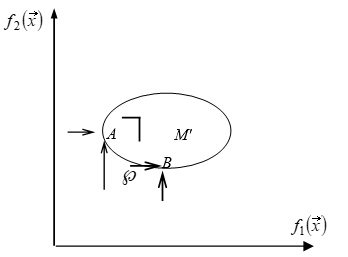
\includegraphics[width=1\linewidth]{pictures/picturefile_6_1}

	Рис. 6.1. Образ множества Парето в плоскости критериев $f_{1}, f_{2}$
\end{center}

Можно сказать, что паретовское решение $\vec{x}^{(0)}$ - это такое решение системы ограничений, для которого нет решений этой системы, доминирующих над $\vec{x}^{(0)}$ по всем критериям. Чаще всего множество $\wp $ гораздо уже множества М. Это видно на следующем примере. Пусть рассматривается задача с двумя критериями $f_{1}(\vec{x})$ и $f_{2}(\vec{x})$. Для каждого значения $\vec{x} \in M$ мы имеем точку на плоскости с координатами $(f_{1}(\vec{x}), f_{2}(\vec{x}))$. Множество всех таких точек обозначим ${M}'$ (рис.6.1). Паретовским решениям отвечают точки дуги $АВ$ границы множества  ${M}'$.

Непосредственное вычисление множества Парето $\wp $  довольно сложно. Часто применяют \textit{эвристические приемы решения многокритериальных задач}. Рассмотрим несколько таких приемов.

\textbf{\textit{1. Способ агрегированного критерия.}} Рассмотрим задачу
\begin{equation*}
\sum_{i=1}^{k}a_{i}f_{i}(\vec{x}) \rightarrow min, \vec{x} \in M,
\end{equation*}
где $a_{i}$ - некоторые неотрицательные числа, называемые весовыми коэффициентами. Они характеризуют  относительную важность критериев. Чем больше число $a_{i}$, тем большую важность придают критерию $f_{i}(\vec{i})$. Если все функции $f_{i}(\vec{i})$ выпуклые и множество М — тоже, то у этой задачи есть точка минимума, и она обязательно принадлежит множеству $\wp $. При этом в качестве точки минимума можно получить любую точку множества  $\wp $ надлежащим  выбором весовых коэффициентов. Выбор этих коэффициентов обычно производится эвристически, например, группой специальных экспертов.

\textbf{\textit{2. Способ главного показателя.}} Здесь эвристически выбирается некоторый главный показатель, например, $f_{1}(\vec{x})$. Его стремятся минимизировать при условии, что $\vec{x} \in M$; кроме того, остальные показатели остаются не больше некоторых приемлемых значений \\ $b_{2}, b_{3}, K, b_{k} \: (f_{i}(\vec{x}) \leq b_{i}, i = 2, 3, K, k )$.При таком подходе все показатели, кроме главного, переводятся в разряд заданных ограничений.

\textbf{\textit{3. Способ последовательных уступок.}}
Этот способ построения компромиссного решения предполагает предварительное расположение целевых функций в порядке убывающей  важности: $f_{1}(\vec{x}), f_{2}(\vec{x}), K, f_{k}(\vec{x})$. Сначала находится решение, обращающее в минимум важнейший показатель $f_{1}(\vec{x})$. Пусть $f_{1min}=b_{1}$. Затем назначается некоторая "уступка" $\bigtriangleup b_{1}$, которую мы согласны сделать для того, чтобы минимизировать второй показатель $f_{2}(\vec{x})$. К первоначальной системе ограничений добавляется условие $f_{1}(\vec{x}) \leq b_{1}+\bigtriangleup b_{1}$ и с новой системой ограничений находится min$f_{2}(\vec{x})=b_{2}$. Затем назначается новая уступка  $\bigtriangleup b_{2}$ и к системе ограничений первого шага добавляется условие $f_{2}(\vec{x}) \leq b_{2}+\bigtriangleup b_{2}$. С новой системой ограничений решается задача на минимум функции $f_{3}(\vec{x})$ и т.д. На последнем шаге к системе ограничений добавляется условие $f_{k-1}(\vec{x}) \leq b_{k-1}+\bigtriangleup b_{k-1}$ и находится min$f_{k}(\vec{x})$. Последняя точка минимума $\vec{x}^{(0)}$ считается решением задачи. Такой способ построения компромиссного решения хорош тем, что здесь видно,  ценой какой "уступки" в одном показателе приобретается выигрыш в другом, и какова величина этого выигрыша. Отметим, что последний способ требует эвристического упорядочивания показателей и  такого же  назначения последовательных уступок.

При любом способе постановки многокритериальной задачи для получения ее конкретного решения требуется вмешательство человеческого сознания для проведения неформализуемых оценок.

\addcontentsline{toc}{subsection}{Контрольные вопросы и задачи для самостоятельного решения}
\subsection*{Контрольные вопросы и задачи для самостоятельного решения}

\begin{enumerate}
\itemКак формулируется общая задача нелинейного программирования? Как можно менять формулировку задачи, оставляя задачу эквивалентной исходной?

\itemДайте определение локального экстремума задачи нелинейного программирования. Что такое глобальный экстремум? Какие задачи называются одноэкстремальными?

\itemКогда задача нелинейного программирования называется задачей на условный экстремум? Что такое функция Лагранжа задачи на условный экстремум? В чем заключаются необходимые условия условного экстремума?

\itemСформулируйте достаточные условия условного экстремума. Что такое критерий Сильвестра и как он используется при выяснении характера стационарной точки функции Лагранжа?

\itemДайте определение выпуклого множества в Rn и выпуклой функции. Что такое задача выпуклого программирования? Является ли такая задача одноэкстремальной?

\itemЧто такое функция Лагранжа задачи выпуклого программирования и ее седловая точка?

\itemСформулируйте теорему Куна-Таккера.

\itemКак формулируются необходимые и достаточные условия Седловой точки?

\itemКак формулируются необходимые и достаточные условия Седловой точки?

\itemКак решить задачу выпуклого квадратичного программирования сведением к вспомогательной задаче линейного программирования?

\itemКак формулируется задача дробно-линейного программирования? Как истолковать эту задачу геометрически в случае двух переменных?
\itemКак сводится задача дробно-линейного программирования к задаче линейного программирования с помощью введения новых переменных?

\itemОпишите метод наискорейшего градиентного спуска для задач на безусловный экстремум. В чем состоит расчетная схема метода Ньютона-Рафсона?

\itemВ чем состоит основная идея метода штрафных функций? Линейная и квадратичная функции штрафа. В чем заключаются преимущества и недостатки каждой из них?

\itemЧто такое паретовское решение многокритериальной задачи? Основные подходы, используемые для решения многокритериальных задач. Что такое способ агрегированного критерия?

\itemОпишите суть способов главного показателя и последовательных уступок.
\end{enumerate}
\newpage
\textit{Используя геометрическое истолкование задачи нелинейного программирования решить задачи 6.1 — 6.4.}
\\
\\
\begin{minipage}{0.4\textwidth}
\zadanie{
	\begin{equation*}
	z = x_{1}x_{2} \rightarrow max,
	\end{equation*}
	\begin{equation*}
	\begin{cases}
	6x_{1}+4x_{2} \geq 12,\\
	2x_{1}+3x_{2} \leq 24,\\
	-x_{1}+4x_{2} \leq 12,\\
	x1, \:\:\: x2 \geq 0.
	\end{cases}
	\end{equation*}
	\textbf{Ответ:} $z_{max}$ = 24, точка max (6; 4).
}

\end{minipage}
\hfill
\begin{minipage}{0.45\textwidth}

\zadanie{
	\begin{equation*}
	z = 9(x_{1}-5)^{2}+4(x_{2}-6)^{2} \rightarrow min,
	\end{equation*}
	\begin{equation*}
	\begin{cases}
	3x_{1}+2x_{2} \geq 12,\\
	x_{1}-x_{2} \leq 6,\\
	-x_{2} \leq 4,\\
	x1, \:\:\: x2 \geq 0.
	\end{cases}
	\end{equation*}
	\textbf{Ответ:} $z_{min}$ = 16, точка min \:\:\:\:\:\: (5; 4).
}
\end{minipage}
\\
\\
\\
\begin{minipage}{0.4\textwidth}

\zadanie{
	\begin{equation*}
	z = 4x_{1}+3x_{2} \rightarrow max,
	\end{equation*}
	\begin{equation*}
	\begin{cases}
	x_{1}^{2}-2x_{1}+x_{2}^{2}-2x_{2}-34 \leq 0,\\
	x_{1} \geq 1,\\
	-x_{2} \geq 1.
	\end{cases}
	\end{equation*}
	\textbf{Ответ:} $z_{max}$ = 37, точка max (5,8;4,6).
}
\end{minipage}
\hfill
\begin{minipage}{0.45\textwidth}

\zadanie{
	\begin{equation*}
	z = x_{1}x_{2} \rightarrow max,
	\end{equation*}
	\begin{equation*}
	\begin{cases}
	x_{1}^{2}+2x_{1}+x_{2}^{2}-2x_{2}-14 \geq 0,\\
	2x_{1}+x_{2} \leq 10,\\
	-x_{1}, \: x_{2} \geq 0.
	\end{cases}
	\end{equation*}
	\textbf{Ответ:} $z_{max}$ = 12,5, точка max (2,5; 5).
}
\end{minipage}
\\
\\
\\
\textit{В задачах 6.5 — 6.8 найти условные экстремумы указанных функций и определить их характер.}
\\
\begin{minipage}{0.4\textwidth}

\zadanie{
	\begin{equation*}
	z = x_{1}^{2}+x_{2}^{2}+x_{3}
	\end{equation*}
	\begin{center}
		при условиях
	\end{center}
	\begin{equation*}
	\begin{cases}
	x_{1}+x_{2}+x_{3}=4,\\
	2x_{1}-3x_{2}=12.
	\end{cases}
	\end{equation*}
	\begin{equation*}
	\textbf{Ответ:}
	\begin{cases}
	z_{min} = 16\frac{53}{64} \: \textit{в точке}\\
	(27/8; -7/4; 19/8).
	\end{cases}
	\end{equation*}
}
\end{minipage}
\hfill
\begin{minipage}{0.45\textwidth}

\zadanie{
	\begin{equation*}
	z = x_{1}x_{2}x_{3}
	\end{equation*}
	\begin{center}
		при условиях
	\end{center}
	\begin{equation*}
	\begin{cases}
	2x_{1}x_{2}+x_{2}x_{3}=4,\\
	2x_{1}-3x_{2}=12.
	\end{cases}
	\end{equation*}
	\begin{equation*}
	\textbf{Ответ:}
	\begin{cases}
	z_{min} = -56/27 \: \textit{в точке}\\
	(-1,3;-26/3;-28/39),\\
	z_{max} = 72 \: \textit{в точке}\\
	(3;-2;-12).
	\end{cases}
	\end{equation*}
}
\end{minipage}

\begin{minipage}{0.4\textwidth}

\zadanie{
	\begin{equation*}
	z = x_{1}x_{2}+x_{2}x_{3}
	\end{equation*}
	\begin{center}
		при условиях
	\end{center}
	\begin{equation*}
	\begin{cases}
	x_{1}+x_{2}=4,\\
	x_{2}+x_{3}=4.
	\end{cases}
	\end{equation*}
	\begin{equation*}
	\textbf{Ответ:}
	\begin{cases}
	z_{max} = 8 \: \textit{в точке}\\
	(2;2;2).
	\end{cases}
	\end{equation*}
}
\end{minipage}
\hfill
\begin{minipage}{0.45\textwidth}

\zadanie{
	\begin{equation*}
	z = 3x_{1}^{2}+2x_{1}+2x_{2}^{2}+4x_{2}x_{3}
	\end{equation*}
	\begin{center}
		при условиях
	\end{center}
	\begin{equation*}
	\begin{cases}
	x_{1}^{2}+2x_{2}^{2}=19,\\
	x_{1}+2x_{2}x_{3}=11.
	\end{cases}
	\end{equation*}
	\begin{equation*}
	\textbf{Ответ:}
	\begin{cases}
	z_{min} = -43 \: \textit{в точах}\\
	(-1;3;2) и (-1;-3;-2).
	\end{cases}
	\end{equation*}
}
\end{minipage}
\\

\textit{Решить задачи выпуклого квадратичного программирования 6.9 — 6.12.}
	\\

\zadanie{
	\begin{equation*}
	f=2x_{1}^{2}+2x_{2}^{2}-x_{1}x_{2}-x{1}-4x_{2} \rightarrow min;
	\end{equation*}
	\begin{equation*}
	\begin{cases}
	x_{1}+2x_{2} \leq 12,\\
	3x_{1}+x_{2} \leq 15,
	\end{cases}
	\end{equation*}
	\begin{equation*}
	x_{1}, \:\:\: x_{2} \geq 0.
	\end{equation*}
	\begin{equation*}
	\textbf{Ответ:}
	f_{min}=-\frac{35}{15} \textit{при} x_{1}=\frac{8}{15}, x_{2}=\frac{17}{15}.
	\end{equation*}
}
\zadanie{
	\begin{equation*}
	f=x_{1}^{2}+x_{2}^{2}-x{1}-8x_{2} \rightarrow min;
	\end{equation*}
	\begin{equation*}
	\begin{cases}
	x_{1}+2x_{2} \leq 7,\\
	x_{2} \leq 5,
	\end{cases}
	\end{equation*}
	\begin{equation*}
	x_{1}, \:\:\: x_{2} \geq 0.
	\end{equation*}
	\begin{equation*}
	\textbf{Ответ:}
	f_{min}=-\frac{65}{4} \textit{при} x_{1}=\frac{1}{4}, x_{2}=4.
	\end{equation*}
}
\zadanie{
	\begin{equation*}
	f=x_{1}^{2}+x_{2}^{2}-2x{1}-8x_{2} \rightarrow min;
	\end{equation*}
	\begin{equation*}
	\begin{cases}
	x_{1}+2x_{2} \leq 12,\\
	-x_{1}+x_{2} \geq -8,
	\end{cases}
	\end{equation*}
	\begin{equation*}
	x_{1}, \:\:\: x_{2} \geq 0.
	\end{equation*}
	\begin{equation*}
	\textbf{Ответ:}
	f_{min}=-16 \: \textit{при} \: x_{1}=0, x_{2}=4.
	\end{equation*}
}
	\newpage

\zadanie{
	\begin{equation*}
	f=x_{1}^{2}+x_{2}^{2}+2x_{3}^{3}-2x_{2}-3x{3} \rightarrow min;
	\end{equation*}
	\begin{equation*}
	\begin{cases}
	x_{1}+x_{2}+x_{3} \leq 18,\\
	x_{2} \leq 12,\\
	x_{1}+2x_{3} \leq 14,
	\end{cases}
	\end{equation*}
	\begin{equation*}
	x_{1}, \:\:\: x_{2}, \:\:\: x_{3} \geq 0.
	\end{equation*}
	\begin{equation*}
	\textbf{Ответ:}
	f_{min}=-\frac{17}{8} \textit{при} x_{1}=0, x_{2}=1, x_{3}=\frac{3}{4}.
	\end{equation*}
}
\textit{Решить задачи дробно-линейного программирования 6.13 — 6.17.}
\\

\zadanie{
\begin{equation*}
z=\frac{-5x_{1}+2x_{2}}{3x_{1}+4x_{2}} \rightarrow max,
\end{equation*}
\begin{equation*}
\begin{cases}
x_{1}+4x_{2}+x_{3} = 16,\\
2x_{1}+3x_{2}-4x_{4} = 12,\\
3x_{1}-2x_{2}+x_{5} = 18,
\end{cases}
\end{equation*}
\begin{equation*}
x_{i} \geq 0 (i = \overline{1, 5}).
\end{equation*}
\begin{equation*}
\textbf{Ответ:}
z_{max}=1/2 \: \textrm{в точке} \: (0; 4; 0; 0; 26).
\end{equation*}
}
\zadanie{
\begin{equation*}
z=\frac{3x_{1}-x_{2}}{x_{1}+x_{2}} \rightarrow max,
\end{equation*}
\begin{equation*}
\begin{cases}
x_{1}+x_{2}-x_{3} = 5,\\
-x_{1}+3x_{2}+x_{4} = 7,\\
3x_{1}-x_{2}+x_{5} = 11,
\end{cases}
\end{equation*}
\begin{equation*}
x_{i} \geq 0 (i = \overline{1, 5}).
\end{equation*}
\begin{equation*}
\textbf{Ответ:}
z_{max}=2,2 \: \textrm{в точке} \: (4; 1; 0; 8; 0).
\end{equation*}
}
\zadanie{
\begin{equation*}
z=\frac{8x_{1}+3x_{2}+2x_{3}+x_{4}}{x_{1}+x_{2}+x_{3}+x_{4}} \rightarrow max,
\end{equation*}
\begin{equation*}
\begin{cases}
2x_{1}+x_{2}+x_{3}+3x_{4} \leq 300,\\
x_{1}+2x_{3}+x_{4} \leq 70,\\
x_{1}+2x_{2}+x_{3} \leq 340,
\end{cases}
\end{equation*}
\begin{equation*}
x_{i} \geq 0 (i = \overline{1, 4}).
\end{equation*}
\begin{equation*}
\textbf{Ответ:}
z_{max}=8 \: \textrm{в точке} \: (70; 0; 0; 0).
\end{equation*}
}
\zadanie{
\begin{equation*}
z=\frac{5x_{1}-x_{2}+8x_{3}+10x_{4}-5x_{5}+x_{6}}{x_{1}+x_{2}+x_{3}+x_{4}+x_{5}+x_{6}} \rightarrow max,
\end{equation*}
\begin{equation*}
\begin{cases}
2x_{1}-x_{2}+3x_{4}+x_{5}-x_{6} = 40,\\
-x_{1}+2x_{2}+x_{3}+2x_{4}+2x_{6} = 20,\\
3x_{1}-x_{}+2x_{3}-x_{4}+3x_{5}+x_{6} = 30,
\end{cases}
\end{equation*}
\begin{equation*}
x_{i} \geq 0 (i = \overline{1, 6}).
\end{equation*}
\begin{equation*}
\textbf{Ответ:}
z_{max}=489/62 \: \textrm{в точке} \: (6,8; 0; 9,2; 8,8; 0; 0).
\end{equation*}
}
\zadanie{
\begin{equation*}
z=\frac{2x_{1}-3x_{2}+4x_{3}+5x_{4}5x_{5}+8x_{6}}{x_{1}+x_{2}+x_{3}+x_{4}+x_{5}+x_{6}} \rightarrow max,
\end{equation*}
\begin{equation*}
\begin{cases}
x_{1}+5x_{2}-3x_{3}-4x_{4}+2x_{5}+x_{6} = 120,\\
2x_{1}+9x_{2}-5x_{3}-7x_{4}+4x_{5}+2x_{6} = 320,
\end{cases}
\end{equation*}
\begin{equation*}
x_{i} \geq 0 (i = \overline{1, 6}).
\end{equation*}
\begin{equation*}
\textbf{Ответ:}
z_{max}=98/13 \: \textrm{в точке} \: (0; 0; 0; 80; 0; 440).
\end{equation*}
}
